\documentclass{article}

\usepackage{url}
\usepackage{graphicx}
\usepackage{subfigure}

\usepackage[utf8]{inputenc}
\usepackage[ngerman]{babel}

\usepackage{booktabs}
\usepackage{multirow}
\usepackage{pifont}
\usepackage{color}
\newcommand{\cmark}{\ding{51}}%
\newcommand{\xmark}{\ding{56}}%
\usepackage{listings}

\definecolor{blue}{rgb}{0,0,1}
\definecolor{violet}{rgb}{0.5,0,0.5} 
\definecolor{darkred}{rgb}{0.5,0,0}
\definecolor{darkblue}{rgb}{0,0,0.75}
\definecolor{darkgreen}{rgb}{0,0.5,0}

\lstset{%
  language=C,%
  morekeywords={constexpr,nullptr,size\_t,this,send,receive,\_\_global,\_\_kernel},%
  basicstyle=\ttfamily\small,%
  sensitive=true,%
  keywordstyle=\color{darkblue},%
  stringstyle=\color{darkgreen},%
  commentstyle=\color{violet},%
  showstringspaces=false,%
  tabsize=4,%
  numberstyle=\footnotesize,%
  xleftmargin=\parindent,%
  moredelim=[is][\color{red}]{|}{|},
  breaklines=true
}

\begin{document}

%don't want date printed
\date{}

\title{Verteilte Systeme Aufgabe 3 Konzept}

\author{
  Marian Triebe, Moritz Heindorf\\
  %Dept. Informatik, HAW Hamburg, Germany\\
  \{marian.triebe, moritz.heindorf\}@haw-hamburg.de
}

\maketitle

\section{Analyse der Aufgabenstellung}
Es ist ein verteiltes Programm zu entwickeln das Sensordaten auf einem vorgegebenen Interface ausgibt.
Das Programm soll in der Lage sein die einzelnen Sensor-Komponenten selbständig zu verwalten, dazu wird ein Wahlalgorithmus verwendet der einen Koordiator bestimmt.
Außerdem soll das Programm erkennen können wenn Sensoren ausfallen, bzw. dazukommen und falls nötig erneut eine Wahl abhalten um einen neuen Koordinator zu bestimmen.
Der Koordinator ist dafür verantwortlich das alle anderen Sensoren zeitgleich ihre Messdaten an das GUI weitergeben und das nicht zwei Sensoren Daten an das selbe GUI-Element liefern.

\section{Aufbau der Programme}
Das Programm soll zur Kommunikation die JAX-WS verwenden daher wird als Programmiersprache Java verwendet. Um die selbst Koordination zu ermöglichen wird der Sensor in zwei verschiedenen Betriebsarten laufen können. In der ersten handelt er als Sensor,
reagiert nur auf die vom Koordinator eingehenden Befehle. Beim Programmstart muss ihm deswegen ein die Adresse eines aktiven Sensors mitgeteilt werden damit er sich bei diesem über den aktuellen Koordinator informieren und anschließend anmelden kann.
Als Koordinator sendet der Sensor periodisch die Aufforderung ihre Daten abzuliefern an die mit der GUI-Anwendung verbundenen Sensoren. Sollte einer der Sensoren nicht auf eine Anfrage reagieren muss der Koordinator die Liste über die aktuell aktiven Sensoren aktualisieren.
Da alle Sensoren eine Liste mit allen verbundenen Sensoren enthalten kann der Bully-Algorithmus als Wahlalgorithmus zur Bestimmung der Koordinators verwendet werden.

\newpage
\subsection{Klassendiagramm}
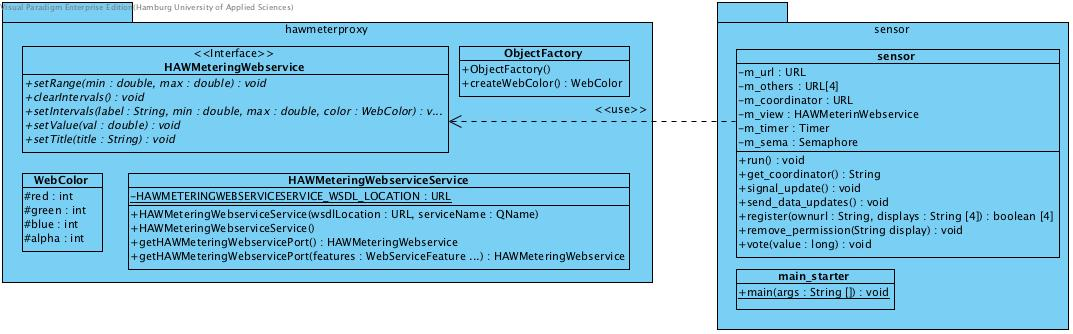
\includegraphics[scale=.35]{documents/classdiagram}

\subsection{Wertigkeit in der Bully-Wahl}
Für die Wertigkeit im Bully-Wahlverfahren haben wir zwei Ideen welche sich eignen würden.
\begin{enumerate}
	\item URL mit String-compare vergleichen, da hier ''kleiner'', ''größer'' sowie ''gleich'' erkannt werden kann
	\item SHA1 Hash über URL und dann einzelne ASCII Zeichen aufaddieren (Wertigkeit)
\end{enumerate}

\section{Mögliche Probleme}
Wir haben keine Probleme gefunden, die sich nicht relativ einfach lösen lassen. Trotzdem listen wir diese kurz auf.
\begin{itemize}
	\item Bei der Wahl besitzen zwei Sensoren die gleiche Wertigkeit
	\item Wie weit muss Thread-Sicherheit von dem zu implementierenden Programm sichergestellt werden
\end{itemize}

\end{document}
